\documentclass{jsarticle}
\usepackage[dvipdfmx]{graphicx}

\title{Information System Analysis 4/15日分レポート}
\author{平田 蓮 \ 6930375031}

\begin{document}
\maketitle

添付したスクリプトを実行した際の出力を以下に示す。

\begin{verbatim}
[1] "stats"
# A tibble: 2 × 4
    Species mean_Nconc sd_Nconc median_Nconc
    <fct>        <dbl>    <dbl>        <dbl>
1 Alder         3.93    0.482         3.95
2 Poplar        2.81    0.380         2.79

[1] "t-test"

    Welch Two Sample t-test

data:  Nconc by Species
t = 14.081, df = 111.82, p-value < 2.2e-16
alternative hypothesis: true difference in means between group Alder and group Poplar 
is not equal to 0
95 percent confidence interval:
    0.9589648 1.2730352
sample estimates:
    mean in group Alder mean in group Poplar 
            3.930333             2.814333 
\end{verbatim}

\paragraph{2種それぞれの窒素濃度の平均、標準偏差、中央値}
    スクリプトの出力より表~\ref{tab:stats}の結果がわかる。

    \begin{table}
        \centering
        \caption{窒素濃度の平均、標準偏差、中央値}
        \label{tab:stats}
        \begin{tabular}{l|rrr} \hline
            種 & 平均 & 標準偏差 & 中央値 \\ \hline\hline
            Alder & 3.93 & 0.482 & 3.95 \\
            Poplar & 2.81 & 0.380 & 2.79 \\ \hline
        \end{tabular}
    \end{table}

\paragraph{2種の窒素濃度を比較するために図示}
    箱ひげ図を図~\ref{fig:box}に示す。
    \begin{figure}
        \centering
        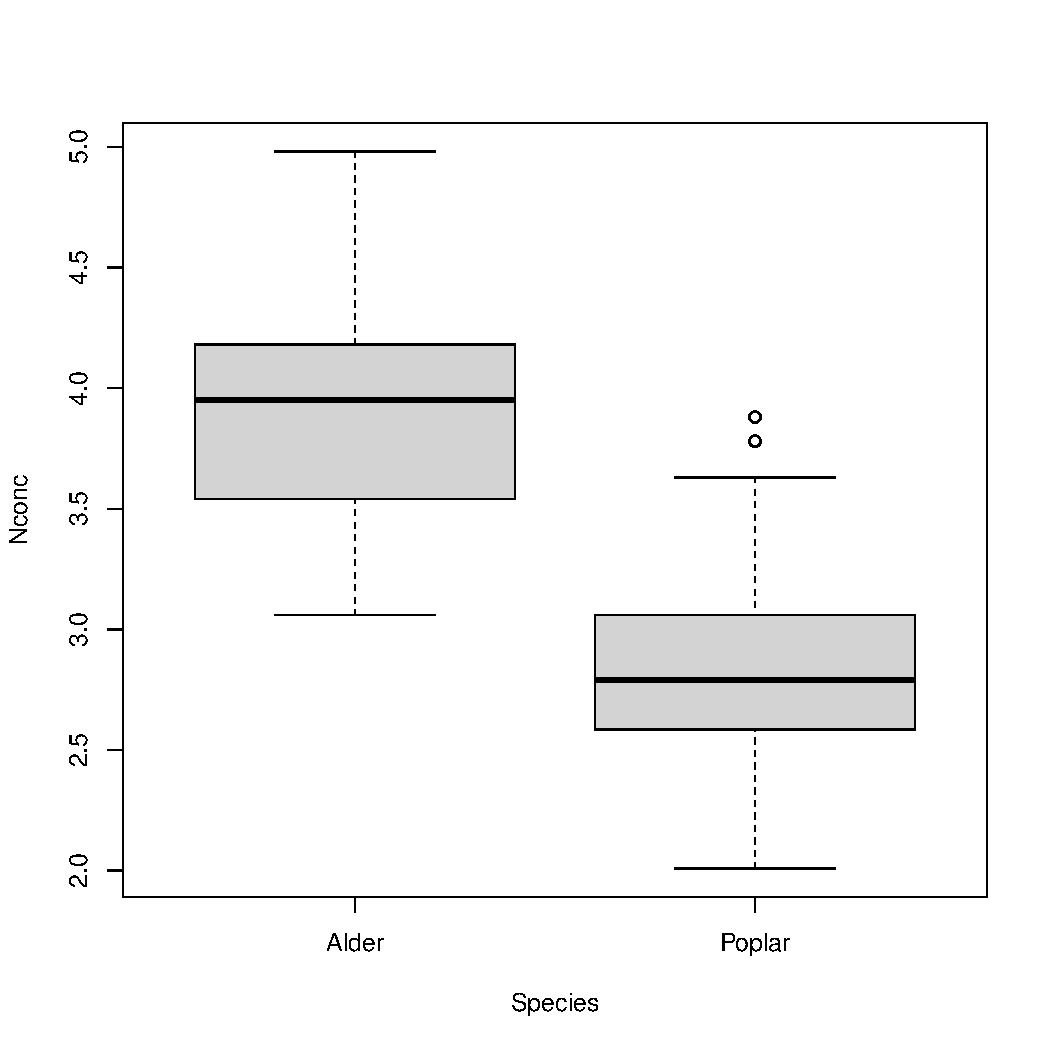
\includegraphics[width=0.6\hsize]{box-chart.pdf}
        \caption{種ごとの箱ひげ図}
        \label{fig:box}
    \end{figure}

\paragraph{2種の窒素濃度間に統計的に差があるか調べる}
    スクリプトの出力より、2種の窒素濃度感に優位差があることがわかる。

\end{document}